\documentclass{article}
\usepackage[german]{babel}
\usepackage[utf8]{inputenc}
% Set title
\def\Title{Smart Factory}
\title{\Title}
\def\Author{Kevin Stahel und Markus Gachnang}
\author{\Author}
\def\Subject{Sind ''Smart Factories'' bereits Realität \\ oder nur ein Konzept auf Papier?}
\date{\today{}}

\PassOptionsToPackage{hyphens}{url}\usepackage{hyperref}
\def\UrlBreaks{\do\/\do-\do:\do.}
\hypersetup{
    colorlinks=true,
    linkcolor=black,
    citecolor=black,
    urlcolor=blue,
	linktoc=all,
    pdftitle={\Title},
    pdfsubject={\Subject},
    pdfauthor={\Author}
}
\usepackage{lastpage}
\usepackage{graphicx}
\usepackage{xcolor}
\usepackage{booktabs}
\usepackage{calc}
% geometry
\usepackage{geometry}
\geometry{a4paper,portrait,left={3cm},right={3cm},top={2cm},bottom={2cm},includehead,head={0.11\textwidth}}
% Colors
\definecolor{LightGray}{rgb}{.96,.92,.90}
\definecolor{Gray}{rgb}{0.79, 0.75, 0.73}
\definecolor{DarkGray}{rgb}{.46,.42,.40}
\definecolor{DarkestGray}{rgb}{.31,.28,.26}

\def\SmartFactory{\textcolor{DarkestGray}{\textit{Smart Factory}}}

% fancyhdr
\usepackage{fancyhdr}
\pagestyle{fancyplain}
\fancyhf{}
% set header/footer
\lhead{
\includegraphics[width=0.2\textwidth]{ost}}
\chead{\textbf{\Title}\\\Author}
\rhead{\small\thepage\hspace{2pt}/\hspace{2pt}\pageref{LastPage}}
% Bibliographie
\usepackage{cite}
\def\BibTeX{{\rm B\kern-.05em{\sc i\kern-.025em b}\kern-.08em
    T\kern-.1667em\lower.7ex\hbox{E}\kern-.125emX}}
% This document uses 'limap'. Inforamtion are available at https://www.ctan.org/pkg/limap
\usepackage[german]{limap}
\usepackage{color}
% The macro \MapBlockLabelFont determines the font changing command to be used for typesetting the block label. The default is empty.
\renewcommand\MapBlockLabelFont{\color{DarkestGray}}
% The macro \MapParskip determines the vertical distance of the text from the separating rules. The default is 2ex.
\renewcommand\MapParskip{1ex}
% The macro \MapTitleFraction determines the part of the page width devoted to the block label area. It is a fraction in the range from 0 to 1. The default value of \MapTitleFraction is 0.2.
\renewcommand\MapTitleFraction{.2}
% This macro determines the part of the page width devoted to the text area. It is a fraction in the range from 0 to 1. The default value of \MapTextFraction is 0.75.
% \MapTitleFraction and \MapTextFraction should add up to something less or equal to 1. Otherwise you will get some “overfull hbox” messages.
\renewcommand\MapTextFraction{.8}
% The macro \MapRuleWidth determines the width of the rules drawn between blocks. It is defined as a macro containig a length. The default is 1pt.
% It can even be set to 0pt to suppress the lines at all
\renewcommand\MapRuleWidth{1pt}
% The macro \MapRuleStart can for instance be used to achieve colored rules. For this purpose we can include the package xcolor in the preamble and select a named color for the rule. 
\renewcommand\MapRuleStart{\color{Gray}}
% The macro \MapTitleFont determines the font changing command to be used when typesetting the title of a map. The default is \Large.
\renewcommand\MapTitleFont{\Large\bfseries}
\renewcommand\MapFont{\normalsize}
% This macro determines the font changing command to be used for typesetting the additional text after titles on followup pages of multi-page maps. The default value is \small.
\renewcommand\MapTitleContinuedFont{\normalsize}
\renewcommand\MapContinued{Fortsetzung}
% Every block in TOC
%\def\MapBlockStartHook{}
%\set\MapBlockStartHook\MapBlockTOC
\usepackage{titlesec}
%%%%%%%%%%%%%%%%%%%%%%%%%%%%%%%%%%%%%%%%%%%%%%%%%%%%%%%%%%%%%%%%%%%%%%%%
\begin{document}
% print title
\begin{titlepage}
  \begin{center}
    \Huge\textbf{\Title}
    \par\bigskip\bigskip
    \large\Subject
    \normalsize
    \par\bigskip\bigskip
  \begin{tabular}{p{3cm} p{6cm}}
    \textcolor{DarkestGray}{Autoren} & \Author\medskip\\
    \textcolor{DarkestGray}{Im Auftrag} & Rhetorische Kommunikation für IngenieurInnen (RheKI), Rolf Murbach\par
\includegraphics[width=0.3\textwidth]{ost}\medskip\\
    \textcolor{DarkestGray}{Datum} & \today\medskip\\
  \end{tabular}
\end{center}
\par\bigskip\bigskip
  \def\svgscale{0.9}
  \input{TitleImage.pdf_tex}
\end{titlepage}

% print index
\begingroup
% Section
\titleformat
{\section} % command
[display] % shape
{\MapTitleFont} % format
{\thesection.} % label
{\MapParskip} % sep
{} % before-code
[\MapTitleContinuedFont] % after-code
  \setcounter{page}{1}
  \tableofcontents{}
\endgroup
%\newpage

%%%%%%%%%%%%%%%%%%%%%%%%%%%%%%%%%%%%%%%%%%%%%%%%%%%%%%%%%%%%%%%%%%%%%%%%
\begin{Map}{Abstract}

\Block{Definition}
Der Begriff \SmartFactory\ kommt von der Hightech-Strategie der deutschen Bundesregierung als Teil des Zukunftsprojekts ''Industrie 4.0''\cite{WasIndustrie40}. Es beschreibt Fertigungsanlagen und Logistiksysteme welche weit möglichst ohne menschliche Komponenten auskommt und somit sich selber verwalten kann\cite{Industrie40TippsUmsetzung}.

\Block{Fragestellung}
Den Begriff von \SmartFactory\ gibt es schon seit 2014, aber gibt es auch Fertigungsanlagen, die der Definition gerecht werden?
Wir versuchen, eine genaue Definition zu erarbeiten, welche unterscheidet, ob es sich bei einer Fertigungsanlage auch um eine \SmartFactory\ handelt.

\Block{Vorgehen}
Bei der Recherche konzentrieren wir uns auf die Definition und Ausarbeitung einer \SmartFactory\ und werden so eine möglichst genaue Checkliste erstellen. Anhand dieser Liste wird man in der Lage sein, eine Fertigungsanlage als \SmartFactory\ zu identifizieren. Die Quellen zur ersten Recherchen sind unter \ref{block:KommentierteQuellenliste} aufgeführt. \par

Anschliessend suchen wir nach Fertigungsanlagen, welche möglichst viele oder gar alle diese Punkte erfüllt. \par

Am Ende ziehen wir eine Schlussvolgerung und werden die Fragestellung beantworten.

\Block{Fazit}
Die Umsetzung einer \SmartFactory\ ist zum heutigen Zeitpunkt, auf Grund technischer Limitierungen, noch nicht vollständig zu erreichen.
Einige Firmen kommen dem Kozept jedoch schon sehr nahe und versuchen aktiv die Ideen der Industrie 4.0 zu nutzen.

\Block{Schlüsselbegriffe}
smart factory, Umsetzung einer Fertigungsanlage, Industrie 4.0


\end{Map}

%%%%%%%%%%%%%%%%%%%%%%%%%%%%%%%%%%%%%%%%%%%%%%%%%%%%%%%%%%%%%%%%%%%%%%%%
\begin{Map}{Checkliste}\label{map:CheckListe}
\Block{Erläuterung}
Wir beschreiben Anhand von verschiedenen Definitionen und Informationen eine Checkliste, welche Ausschlag gibt, ob eine Fertigungsanlage nach unseren Recherchen als \SmartFactory\ definiert werden kann.

\Block{Liste}
\begin{tabular}{p{2.5cm}p{8cm}}\toprule
	Schlagwort 
	& Beschreibung \\\midrule
	
	\hypertarget{CheckListe:Logistik}{Logistik}
	& Kann selbständig fehlende Materialien organisieren und Inventar managen.\cite{WasIndustrie40} \\\midrule
	
	\hypertarget{CheckListe:AnpassbareProdukte}{Anpassbare Produkte}
	& Produkte können dynamisch angepasst werden, so das zum Beispiel Farbe und Ausstattung vom Kunden bestimmt werden kann.\cite{WasIndustrie40} \\\midrule
	
	\hypertarget{CheckListe:SmartProduct}{Smart Products}
	& Daten zum Ablauf der Produktion und zum Zustand eines Produkts werden zusammengeführt und ausgewertet. Das Produkt kann identifiziert und nachverfolgt werden. \cite{Industrie40TippsUmsetzung} \\\midrule
	
	\hypertarget{CheckListe:Fertigungsprozess}{Fertigungsprozesse automatisiert}
	& Die Anlage erzeugt eigenständig die Produkte. Der Mensch hat die Vorgänge nur zu kontrollieren und zu optimieren. Er ist nicht Teil des Fertigungsprozesse sondern ein Controller.\cite{REFA}\\\bottomrule
	
\end{tabular}
\Block{}
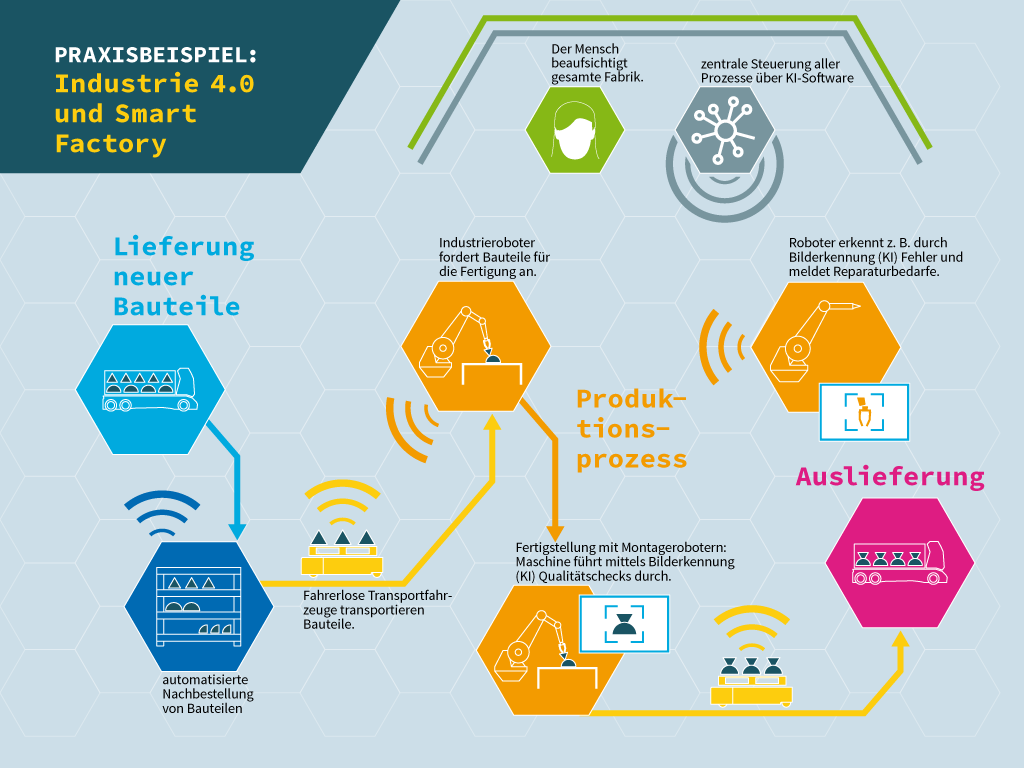
\includegraphics[scale=0.33]{grafik}
\end{Map}

%%%%%%%%%%%%%%%%%%%%%%%%%%%%%%%%%%%%%%%%%%%%%%%%%%%%%%%%%%%%%%%%%%%%%%%%
\begin{Map}{Fertigungsanlagen}\label{map:Fertigungsanlagen}
\Block{Erläuterung}
Hier listen wir Fertigungsanlagen auf und wenden die \ref{map:CheckListe} an.

\Block{Produktiv}
Viele Hersteller lassen sich nicht in die Karten schauen und geben nur wenig Informationen preis, wie ihre Fertigung realisiert ist. 
\par\medskip
\begin{tabular}{p{3.2cm}p{8cm}}\toprule
  Auto / Audi & Audi behauptet, beim Thema \SmartFactory\ vorne mit dabei zu sein und gibt an, dass sie ihre Fabriken auf den neusten Stand der Dinge bringen. Tatsächlich sieht man, das vieles bereits automatisiert ist, jedoch erkennt man, das gewisse Arbeitsschritte immer noch von Hand erledigt werden müssen und somit den Punkt \hyperlink{CheckListe:Fertigungsprozess}{''Fertigungsprozesse automatisiert''} nicht erfüllen.\cite{Audi}\cite{AudiKommentarlos}\\\midrule
  Blechbearbeitung / Trumpf & Der Werkzeugmaschinenhersteller Trumpf hat in Chicago eine Fertigungsanlage errichtet, die nach eigenen Aussagen einer \SmartFactory\ entspricht. Die Produktionsstrasse von Trumpf ist in der Lage individuelle angepasste Bleichteil vollautomatisch zu bearbeiten und dabei alle relevanten Daten aufzuzeichnen und einer Kontrollperson zur Verfügung zu stellen. Damit scheinen sie unsere Punkte \hyperlink{CheckListe:Fertigungsprozess}{''Smart Products''}, sowie \hyperlink{CheckListe:Fertigungsprozess}{''Fertigungsprozesse automatisiert''} umgesetzt zu haben. Es ist jedoch nicht fest zu stellen in welchem Ausmass die  Punkte erfüllt werden. Bei unseren anderen beiden Punkte \hyperlink{CheckListe:Fertigungsprozess}{''Logistik''} und \hyperlink{CheckListe:Fertigungsprozess}{''Anpassbare Produkte''} kommuniziert Trumpf nur wenige Informationen, aus denen wir jeodch erkennen, dass sie noch nicht vollständig Umgesetzt werden konnten.\cite{Cicago}\cite{Automationspraxis}\\\bottomrule
\end{tabular}

\Block{Experimentell}
Einige Universitäten und Forschungszentren haben experimentelle \SmartFactory s geschaffen.
\par\medskip
\begin{tabular}{p{3.2cm}p{8cm}}\toprule
  Helmut-Schmidt-Universität & Die Helmut-Schmidt-Universität hat unter der Leitung der Handelskammer Hamburg zu Forschungszwecken eine Modellumsetzung einer \SmartFactory\ entwickelt. Es handelt sich dabei um eine Fertigungsanlage, bei der verschiedene simple Zylinder produziert werden können. Es ist jedoch unklar, ob die der Punkt  \hyperlink{CheckListe:Fertigungsprozess}{''Logistik''} umgesetzt werden konnte und auch beim Punkt \hyperlink{CheckListe:Fertigungsprozess}{''Anpassbare Produkte''} muss man davon ausgehen, dass das Modell wenig bis gar nicht flexibel ist und somit den Punkt nur Teilweise erfüllt. Es ist ebenfalls zu beachten das nicht gewehrleistet ist, dass alle Punkte noch erfüllt sind, wenn das System auf die Grösse einer realen Produktionsanlage skaliert wird.\cite{UniSchmidt}\\\midrule
  TODO & TODO: Gachnang\\\bottomrule
\end{tabular}

\Block{Spiele}
TODO Gachnang: Zu Text\par
Das Konzept der \SmartFactory\ ist auch in der Spielindustrie angelangt, so gibt es einige Spiele, in welchen man eine \SmartFactory\ realisieren muss.
\par\medskip
\begin{tabular}{p{3.2cm}p{8cm}}\toprule
  Factorio / \par Satisfactory & Man baut eine Fertigungsanlage um genügend Produkte zu produzieren um den fremden Planeten in einer Rakete verlassen zu können. \par Die beiden Spiele erfüllen nur \hyperlink{CheckListe:Fertigungsprozess}{''Fertigungsprozesse automatisiert''}. Zur Logistik wird solange produziert, wie Material vorhanden ist. Ist zu viel Material vorhanden, staut es sich.\par Produkte sind nicht anpassbar oder Smart.. \\\midrule
  Autonauts & Man muss Robotern kleinere Aufgaben einprogrammieren, um eine Stadt aufzubauen und zu versorgen. \par Wird Material gebraucht, wird dies geholt, je nach Bedingung wird nicht weiter produziert. Hier wird \hyperlink{CheckListe:Logistik}{''Logistik''} und \hyperlink{CheckListe:Fertigungsprozess}{''Fertigungsprozesse automatisiert''} erfüllt, die Produkte sind aber nicht anpassbar oder smart. \\\bottomrule
\end{tabular}
\end{Map}

%%%%%%%%%%%%%%%%%%%%%%%%%%%%%%%%%%%%%%%%%%%%%%%%%%%%%%%%%%%%%%%%%%%%%%%%
\begin{Map}{Schlussfolgerung}
\Block{Erläuterung}
Anhand der \ref{map:CheckListe} und der gefundenen \ref{map:Fertigungsanlagen} können wir nun unsere Fragestellung, ob es bereits \SmartFactory s eingesetzt werden, beantworten. \par

\Block{Diskussion}
Die \SmartFactory\ als Konzept für eine Weiterentwicklung der klassischen Fertungsanlage hat zweifelsohne das Intresse vieler Produktionsfirmen geweckt. Zahlreiche Unternehem bemühungen sich die Ideen der Industrie 4.0 und damit auch der \SmartFactory\ in ihre Produktion aufzunehmen oder zumindest darauf hinzuarbeiten. Die Umsetzung ist jedoch nicht einfach, da die benötigte Technik und ihre Vernetzung noch immer im Forschungsstadium sind. Verschiedenste Universitäten stellen Forschungen zum Thema \SmartFactory\ an und einige bauen sogar eigene Modelle, um die Schwirigkeiten einer Umsetzung zu studieren. Auch Spieleentwickler haben sich an \SmartFactory s\ versucht, aber selbst im Virtuellen wurde eine vollständige Umsetzung nicht erzielt. 

\Block{Schlussfolgerungen}
Aus unseren Recherchen und dem Vergleichen einiger Beispiel mit unserer erarbeiteten Checkliste wird klar, dass obwohl intensiv daran gearbeitet wird, eine vollständige Umsetzung einer \SmartFactory\ noch nicht komplett gelungen ist. Es gibt mehere Gründe, welche einer vollständigen Umsetzung noch weg stehen. Einer der wichtigsten ist, dass das Zusammenbringen und Vereinen der ganzen benötigen Technik hoch komplex ist und deswegen eine enormen Planungsaufwand erfordert. Die Technik selbst stellt auch ein grosses Hindernis dar, da gewisse Arbeiten momentan noch zu kompliziert für Maschienen sind. 
\end{Map}

%%%%%%%%%%%%%%%%%%%%%%%%%%%%%%%%%%%%%%%%%%%%%%%%%%%%%%%%%%%%%%%%%%%%%%%%
\begin{Map}{Quellenverweis}
\Block{Verwendete Verweise}
Dieser Bereich beschreibt Quellen und Referenzen aus dem verfassten Text.

\begingroup
% Remove Titles eg "Literatur"
\renewcommand{\section}[2]{}%
% Reminder: Recreate "SmartFactory.bll" when "citavi/citavi.bib" gets changed => run BibTeX ([F11] in TexMaker)
\bibliography{citavi/citavi}
% Use the "IEEE standard" as style => "IEEEtran.bst"
\bibliographystyle{IEEEtran}
\endgroup
\medskip\medskip\medskip\medskip\medskip\medskip\medskip\medskip\medskip\medskip\medskip
\medskip\medskip\medskip\medskip\medskip\medskip\medskip\medskip\medskip\medskip\medskip
\medskip\medskip\medskip\medskip\medskip\medskip\medskip\medskip\medskip\medskip\medskip
\medskip\medskip\medskip\medskip\medskip\medskip\medskip\medskip\medskip\medskip\medskip
\medskip\medskip\medskip\medskip\medskip\medskip\medskip\medskip\medskip\medskip

\Block{Kommentierte Quellenliste}\label{block:KommentierteQuellenliste}
Im Zuge der ersten Recherchen wurde eine kommentierte Quellenliste erstellt, um als Ausgangspunkt der weiteren Untersuchungen des Themas zu fungieren. Diese Liste verschafft einem einen Überblick über das Thema von \SmartFactory. \\\medskip
\WideBlock{
\begin{tabular}{p{0.2cm}p{4.2cm}p{2cm}p{3.2cm}p{3.2cm}}\toprule
   & Quelle & Art & Inhalt & Eignung \\\midrule

 1 & 
 \url{https://www.plattform-i40.de/PI40/Navigation/DE/Industrie40/WasIndustrie40/was-ist-industrie-40.html} &
 Internet-Dokument / Filmdokument &
 Definition von ''Industrie 4.0'' vom Bundesministerium für Bildung und Forschung von Deutschland &
 Gibt einen Überblick von ''Industrie 4.0'' und den Zusammenhang zu \SmartFactory\\\midrule

 2 &
 Huhmann A., ''Industrie 4.0: Auf dem Weg zur wirklich smarten Factory'' entwickler.de - S\&S Media Support GmbH, 2019. \url{https://entwickler.de/online/iot/industrie-4-0-auf-dem-weg-zur-smart-factory-579911790.html} &
 Internet-Dokument / Zeitschriften-artikel &
 Stand der Dinge und Ausblick auf Industrie 4.0 &
 Beschreibt wie die \SmartFactory\ Wirklichkeit werden und wie der aktuelle Stand der Dinge ist\\\midrule

 3& 
 Limited, Wipro, “In 5 Schritten zum Smart Manufacturing | MoreThanDigital,” MoreThanDigital, 2020. \url{https://morethandigital.info/in-5-schritten-zum-smart-manufacturing/} &
 Internet-Dokument / Zeitschriften-artikel & 
 Beschreibt das Vorgehen in 5 Schritten um zur ''Smart Manufacturing'' zu gelangen & 
 Gibt Definitionen zu \SmartFactory\ und eingesetzte Hilfsmittel um eine solche aufzubauen \\\midrule
 
 4& 
 RICHARDS, G. and Grinsted, S., The logistics and supply chain toolkit: Over 100 tools for tansport, warehousing and inventory manageme, Third edition. ISBN: 9781789660852 & 
 Buch (Monographie) & 
 Beschreibt wie Logistik und Inventar gemanagt werden kann & 
 Gibt unter anderem auch Auskunft, wie dies vollautomatisch (wie in einer \SmartFactory) realisiert werden kann\\\midrule
\end{tabular}}

\WideBlock{
\begin{tabular}{p{0.2cm}p{4.2cm}p{2cm}p{3.2cm}p{3.2cm}}\toprule
   & Quelle & Art & Inhalt & Eignung \\\midrule
   
 5& 
 B. Meussen, „Anwendung von Industrie 4.0 in Forschung und Praxis“, Nordakademie - Hochschule der Wirtschaft, Elmshorn, Arbeitspapiere der Nordakademie 2015–03,  2015. [Online]. Verfügbar unter: \url{http://hdl.handle.net/10419/121298} & 
 Paper & 
 Stand der Dinge und Perspektiven für die Zukunft für die Industrie 4.0 & 
 Beschriebt den aktuellen Stand der Dinge und zeigt Perspektiven für die Zukunft auf\\\midrule
 
 6& 
 T. Ionescu und M. Merz, „Cyber-physische Produktion: Modelle und Inszenierung der Smart Factory“, AIS-Studien, 2018, doi: 10.21241/SSOAR.64876 &
 Paper & 
 Entwicklung eines \SmartFactory\ Demonstrators in einem Grossunternehmen & 
 Zeigt potenzielle Problem beim Schritt in Richtung smart factory für Unternehmen auf\\\midrule
 
 7& 
 T. Schulz und Vogel Business Media GmbH \& Co. KG, Industrie 4.0 Potenziale erkennen und umsetzen. 2017 &
 Buch & 
 Befasst sich mit dem Potential und der Konkreten Umsetzung einer Industrie 4.0 & 
 Detaillierte Analyse des Potentials und möglichen konkreten Umsetzungen einer Industrie 4.0\\\midrule
 
 8& 
 H. S. Kang u. a., „Smart manufacturing: Past research, present findings, and future directions“, Int. J. of Precis. Eng. and Manuf.-Green Tech., Bd. 3, Nr. 1, S. 111–128, Jan. 2016, doi: 10.1007/s40684-016-0015-5 & 
 Paper & 
 Notwenidge Technoligien werden identifiziert und Zukunftsausblicke werden gegeben & 
 Zeigt Notwendigkeiten auf und beschriebt Konzepte für eine Umsetzung auf\\\midrule
 
 9& 
 \url{https://www.youtube.com/watch?v=z7R8jg4Texw} &
 Filmdokument & 
 Erklärt die Funktionnsweise und gibt gibt Einblicke in eine Laborumsetzung einer \SmartFactory & 
 Gibt Einblick in eine praktische Umsetzung des Prinzips im kleinen Rahmen\\\midrule
 
10&
Innovator's Guide Switzerland, die erste Schweizer Test- und Demo-Fabrik zum Thema Industrie 4.0 \url{https://innovators-guide.ch/2017/05/eroffnungsfeier-swiss-smart-factory-die-erste-schweizer-test-und-demo-fabrik-zum-thema-industrie-40/} &
Internet-Dokument / Zeitungsartikel & 
Beschreibt die Eröffnung einer swissmade Smart Factory Demo-Fabrik & 
\SmartFactory -Demo in der Schweiz, eignet sich nur schon dadurch, schweizerisch zu sein (''Hop Schwitz!'') \\\bottomrule
\end{tabular}}

\end{Map}
\end{document}
